\section{AWStream}

\begin{frame}{Fidelity vs.\,Freshness}
  \vspace{2em}
  \begin{figure}
    \centering
    \includegraphics[width=0.8\columnwidth]{figures/fidelity-freshness.pdf}
    \caption{The trade-off space between data freshness and fidelity when facing
      insufficient bandwidth.}
  \end{figure}
\end{frame}

\begin{frame}{Bandwidth-Accuracy Tradeoff}
  \begin{figure}
    \centering
    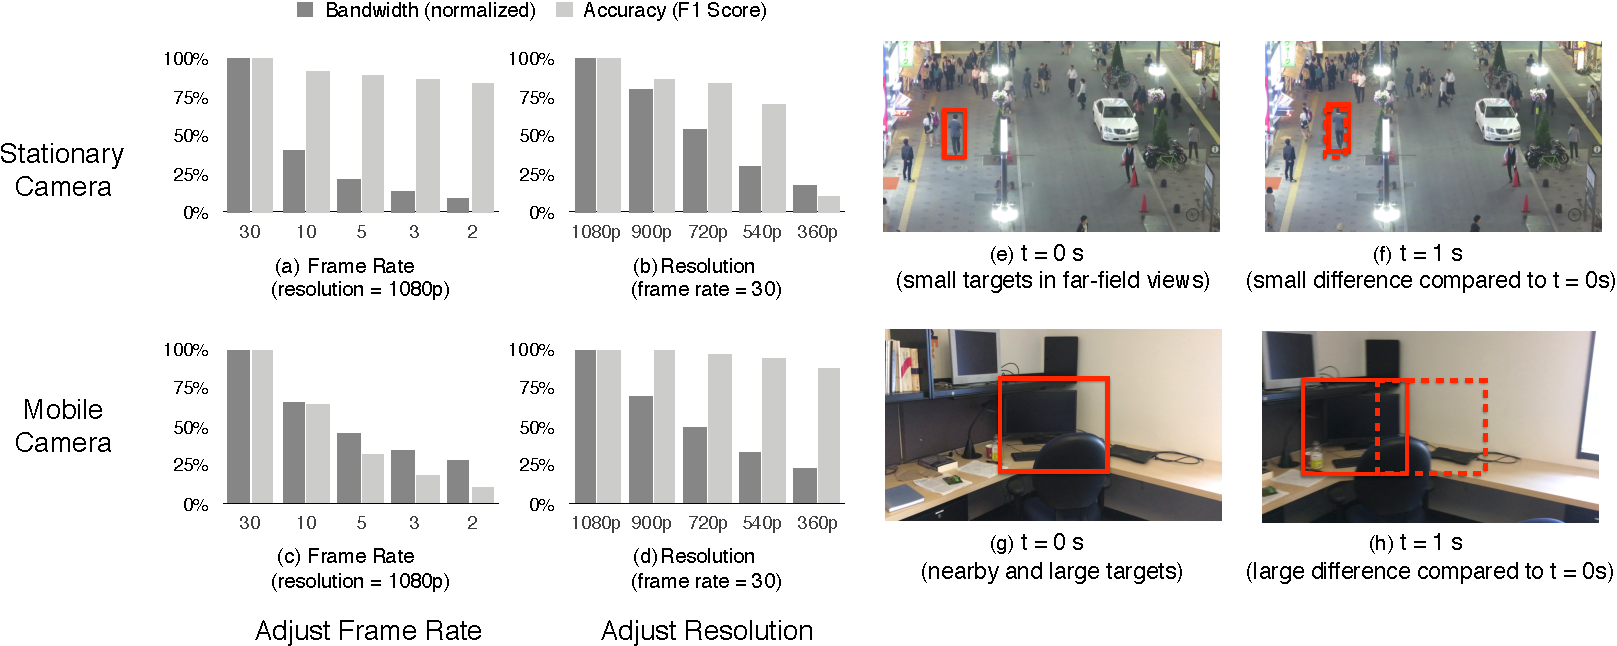
\includegraphics[width=0.85\linewidth]{figures/motiv-app-specific.pdf}
    \caption{The measured bandwidth and application accuracy for two video
      analytics applications. (1) Manual policies lack precision without
      measurements and need to handle multiple dimensions (as in a-d). (2)
      Application-specific optimizations do not generalize: degrading frame rates
      works well for stationary camera (a), but not for mobile camera (c). (e-h)
      shows example frames.}
    \label{fig:app-specific}
  \end{figure}
\end{frame}

\begin{frame}{API}
  \begin{table}
    \scriptsize
    \begin{tabular}{ c r l }
      \toprule
      \multirow{4}{*}{Normal}
      & \textit{map} (f: I $\Rightarrow$ O) & Stream<I> $\Rightarrow$ Stream<O> \\
      & \textit{skip} (i: Integer) & Stream<I> $\Rightarrow$
                                     Stream<I> \\
      & \textit{window} (count: Integer, f: Vec<I> $\Rightarrow$ O) & Stream<I> $\Rightarrow$
                                                                      Stream<O> \\
      & ... & ... \\
      \midrule
      \multirow{5}{*}{Degradation}
      & \textit{maybe} (knobs: Vec<T>, f:  (T, I) $\Rightarrow$ I) & Stream<I> $\Rightarrow$
                                                                     Stream<I> \\
      & \textit{maybe\_skip} (knobs: Vec<Integer>) & Stream<I> $\Rightarrow$ Stream<I> \\
      & \textit{maybe\_head} (knobs: Vec<Integer>) & Stream<Vec<I>{}> $\Rightarrow$
                                                     Stream<Vec<I>{}> \\
      & ... & ... \\
      \bottomrule
    \end{tabular}
  \end{table}
\end{frame}

\begin{frame}[fragile]{\texttt{maybe(knobs: Vec<T>, f: (T, I) => I)}}
  \begin{lstlisting}
let quantized_stream = vec![1, 2, 3, 4].into_stream()
    .maybe(vec![2, 4], |k, val| val.wrapping_div(k))
    .collect();
  \end{lstlisting}
  Output: [1, 2, 3, 4] (no degradation), [0, 1, 1, 2] (k=2), or [0, 0, 0, 1]
  (k=4).

  \pause
  \vspace{2em}
  \begin{lstlisting}
let app = Camera::new((1920, 1080), 30)
    .maybe_downsample(vec![(1600, 900), (1280, 720)])
    .maybe_skip(vec![2, 5])
    .map(|frame| frame.show())
    .compose();
  \end{lstlisting}

\end{frame}

\begin{frame}{Applications}
  \begin{table}
    \footnotesize
    \centering
    \begin{tabular}{c c c c}
      \toprule
      Application & Knobs & Accuracy & Dataset \\
      \midrule
      \specialcell{Augmented\\Reality}
                  & \specialcell{resolution \\ frame rate \\ quantization }
                  & F1 score~\cite{Rijsbergen:1979:IR:539927}
                          & \specialcell{iPhone video clips\\training: office (24
      s)\\testing: home (246 s)} \\
      \midrule
      \specialcell{Pedestrian\\Detection}
                  & \specialcell{resolution \\ frame rate \\ quantization }
                  & F1 score
                          & \specialcell{MOT16~\cite{milan2016mot16}\\training: MOT16-04\\testing: MOT16-03} \\
      \midrule
      \specialcell{Log Analysis\\(Top-K, K=50)}
                  & \specialcell{head (N) \\ threshold (T) }
                  & \specialcell{Kendall's $\tau$~\cite{abdi2007kendall}}
                          & \specialcell{\href{https://www.sec.gov}{SEC.gov} logs~\cite{edgarlog} \\ training: 4 days \\
      testing: 16 days} \\
      \bottomrule
    \end{tabular}
    \vspace{0.5em}
    \caption{Application details.}
    \label{tab:apps}
    \vspace{-1em}
  \end{table}
\end{frame}

\begin{frame}{Runtime Adaptation}
  \begin{figure}
    \centering
    \includegraphics[width=\linewidth]{figures/runtime-adaptation.PDF}
    \caption{Runtime adaptation system architecture.}
    \label{fig:runtime}
  \end{figure}
\end{frame}

\begin{frame}{Profiles}
  \begin{figure}
    \includegraphics[width=\linewidth]{figures/profile-mot.PDF}
  \end{figure}
\end{frame}


%%% Local Variables:
%%% mode: latex
%%% TeX-master: "talk"
%%% TeX-engine: xetex
%%% End:
